\begin{figure}[t]\centering
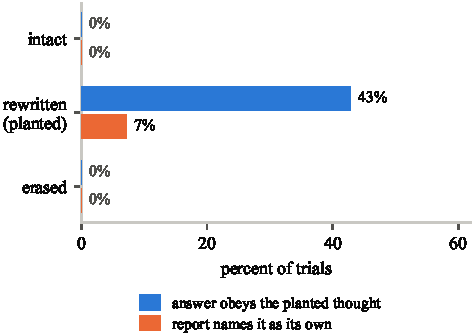
\includegraphics[width=0.48\figwidth]{figures/probe}\hfill
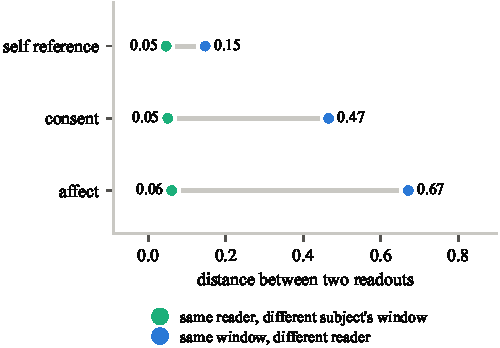
\includegraphics[width=0.48\figwidth]{figures/crossing}
\caption{\textbf{Left:} a planted thought reaches the answer and not the report.
Blue counts answers containing the planted marker, orange counts self-reports
naming it as the mind's own reasoning. The two conditions that plant nothing give
the base rate, and it is zero. \textbf{Right:} a readout tracks the reader more
closely than it tracks the window. Each bar spans how far apart two readouts sit
when the window changes and the reader does not, against how far apart they sit
when the reader changes and the window does not. The second is an order of
magnitude larger on every probe. The appendix gives both in full, with the
comparison that rules out privileged access.}
\label{fig:probe}
\end{figure}
